\section{Evaluation of Results}
\label{cha:evaluation}
\subsection{Tweet Collection}
\label{sec:methodology:data-collection}

Several portions of this paper required collecting data from Twitter.  To
determine the posting rate of tweets of each length, it was necessary to collect
tweets from real accounts.  Therefore, data from
verified\footnote{\url{https://support.twitter.com/articles/119135-faqs-about-verified}
\url{-accounts}}
Twitter accounts was collected.  A verified account is an account that Twitter
has manually verified to be a specific person or brand.  By using verified accounts, this
prevents obtaining data from other bots or fake accounts.  However, it has been
noted that verified accounts may not be a perfect representation of the average
Twitter user, who is not generally a brand or celebrity.  User information stored
includes the username and user ID, a unique integer that Twitter stores for
each user.  A total of 54,114 users were collected.  Additionally, for
creating the Markov chain, tweet content was parsed using a regular expression
from the collected tweets to find username references in the tweets.  In a
tweet, usernames are preceded by an @ symbol.

From the collected user IDs, tweet content, length, unique identifier, and
posting time were collected.  Because of the number of collected users and
the number of tweets posted by each user, during the data collection we only
obtained tweets from 3,709 users.  However, this totaled 7,345,681 tweets.
This data collection was done automatically from a list of verified users that
was obtained from Twitter.  Twitter has a special account with username
\emph{verified} that will follow all verified accounts.  Therefore, we were
able to search for all accounts followed by that special account using the
Twitter API and then begin obtaining tweets posted by each of those accounts.
Not all accounts post in English, some collected data is in other languages
including Portuguese, Spanish, Japanse, and Arabic among others.  In order
to remove these languages, we used the third-party Java library
NGramJ\footnote{\url{http://ngramj.sourceforge.net/index.html}}, which performs
language recognition using n-grams.  An n-gram is a sequence of symbols of length
$n$.  For example, in English a common bigram (2-gram) is \emph{th}.  This library
ranked each tweet according to which language it most resenbled.  We kept only the
tweets where the highest ranking language is English.  This left us with 5,461,009
tweets out of the original 7,345,681.  However, this method is not perfect.
Tweets contain some non-typical English characters in hashtags, names,
misspellings, URLs, etc.  Because of this, the n-gram analysis likely had some
false positives and false negatives.  For example, one tweet had the text
``Vancouver, 9/25'', but the n-gram model marked it as French.  After this
n-gram analysis, tweets were further restricted by checking the character
values in each tweet.  If a tweet contains too many non-ASCII characters,
then it is not likely to be English.  In this case, we removed all tweets that
were 10\% or more non-ASCII characters.  This allows up to approximately 14
non-ASCII characters in a full length tweet.  The final tweet count is 5,011,973.

\subsection{Stego System Evaluation}
\label{sec:evaluation:twittercc}

\subsubsection{Emulab Performance and Reliability Experiment}
\label{subsec:evaluation:twittercc:emulab}

Emulab \cite{emulab-rigorous} is a network testbed and software system designed for testing networked
systems.  It allows experimenters to request a set of physical machines,
or nodes, that
are configured in a specific network configuration as defined by a script
file supplied to the Emulab website.  

The experiment for this paper was performed by generating symbols from a test
alphabet (the English alphabet) and posting
generated tweets using a random text generator and a constructed encoding map.
The input symbols were chosen probabilistically with the weight associated with
their letter frequencies.
The ``botmaster'' acted from a desktop computer outside of the Emulab environment
posting the tweets while the ``bots'' acted from inside an Emulab experimental
setup.  There were five bots in the experiment running Emulab's
\ttf{UBUNTU12-64-STD} operating system image.  The botmaster generated a new
symbol and posted the corresponding tweet every 30 seconds while the bots
performed an HTTP request to the correct Twitter account every 10 seconds
checking for new tweets.  Each time the botmaster posted, it is recorded
to a log file.  Each time the bots read a tweet, they also recorded to a log
file.  Afterwards, the logs were collected to compare the post time with
the retrieval time and also to match each original input symbol with the
decoded symbols from the bots.  Due to a time zone difference between the
botmaster machine and the bots in the Emulab setup, the original time stamps
from the bots appeared one hour later, so one hour was subtracted from their
times when comparing the difference in posting and reading time between the
botmaster and bots.  Figure \ref{fig:evaluation:twittercc:emulab:emulab}
shows the network configuration for the experiment. 

\begin{figure}
\centering
\resizebox {\columnwidth} {!} {
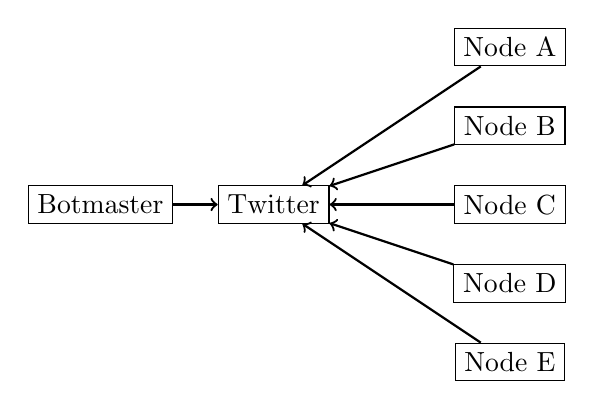
\begin{tikzpicture}
    \node[draw] (botmaster) {Botmaster};
    \node[draw] (twitter) [right of=botmaster,node distance=2.2cm] {Twitter};

    \node[draw] (nodec) [right of=twitter,node distance=3cm] {Node C};
    \node[draw] (nodeb) [above of=nodec,node distance=1cm] {Node B};
    \node[draw] (nodea) [above of=nodeb,node distance=1cm] {Node A};
    \node[draw] (noded) [below of=nodec,node distance=1cm] {Node D};
    \node[draw] (nodee) [below of=noded,node distance=1cm] {Node E};

    \draw[->,thick] (botmaster) -- (twitter);
    \draw[->,thick] (nodea) -- (twitter);
    \draw[->,thick] (nodeb) -- (twitter);
    \draw[->,thick] (nodec) -- (twitter);
    \draw[->,thick] (noded) -- (twitter);
    \draw[->,thick] (nodee) -- (twitter);
\end{tikzpicture}
}
\caption{Diagram for the Emulab experiment network layout.}
\label{fig:evaluation:twittercc:emulab:emulab}
\end{figure}

In the experiment, 100\% of input symbols were correctly decoded by the bots
except for a small set that were off by one.  After examining the data it was
determined that in these cases, the tweets being posted were generated with
a trailing space that was then trimmed by Twitter while posting.  If the tweets
had been generated without spaces, this would not have occurred and so these
cases were dropped from the results.  The average read time in seconds for
each node are shown in table \ref{tab:evaluation:twittercc:emulab:average-read}.
Each node averaged just over five seconds from the botmaster's post to the
bot's read.  This is likely due to the synchronization issues of the botmaster's
posting and the bot's sleep time between reads.  A total of 305 tweets were posted
for this test and 10 of them were dropped for having trailing whitespace.  With
an average transmission time of less than six seconds, the overall transmission
rate is up to 10,800 bytes per day.

\begin{table}
\centering
\begin{tabular}{|c|c|c|c|c|}
    \hline
    Node A & Node B & Node C & Node D & Node E \\
    \hline
    5.725  & 5.644  & 5.600  & 5.912  & 5.888 \\
    \hline
\end{tabular}
\caption{Average read time in seconds for each node.}
\label{tab:evaluation:twittercc:emulab:average-read}
\end{table}

\subsubsection{Capacity}
\label{subsec:evaluation:twittercc:capacity}

There are three major criteria
for stego system evaluation: capacity, steganographic security, and
robustness \cite{steganalysis}.

At the most basic level, the devised stego system can be used to transmit
at most seven bits of information per tweet because a tweet can have a length of
at most 140.  If eight bits were to be transmitted, there would be 256 different
values.  With seven bits, there are 128 different values, so each value can be
sent with a different length tweet.  Therefore, we can state the maximum capacity
as seven bits per tweet.  Tweets are posted to Twitter using UTF-8, which is
a variable length character encoding scheme that is a superset of the ASCII
characters.  UTF-8 characters range from one to four bytes \cite{rfc3629}.
Therefore, the embedding rate will vary depending not only on the length
of the tweet in characters, but also on how many characters per byte are being
used.  The total number of bytes in a tweet is 560, so the total number of
bits is then 4480.  The possible embedding rates are shown in figure
\ref{fig:evaluation:twittercc:capacity:emebedding-rate}.

\begin{figure}
    \centering
    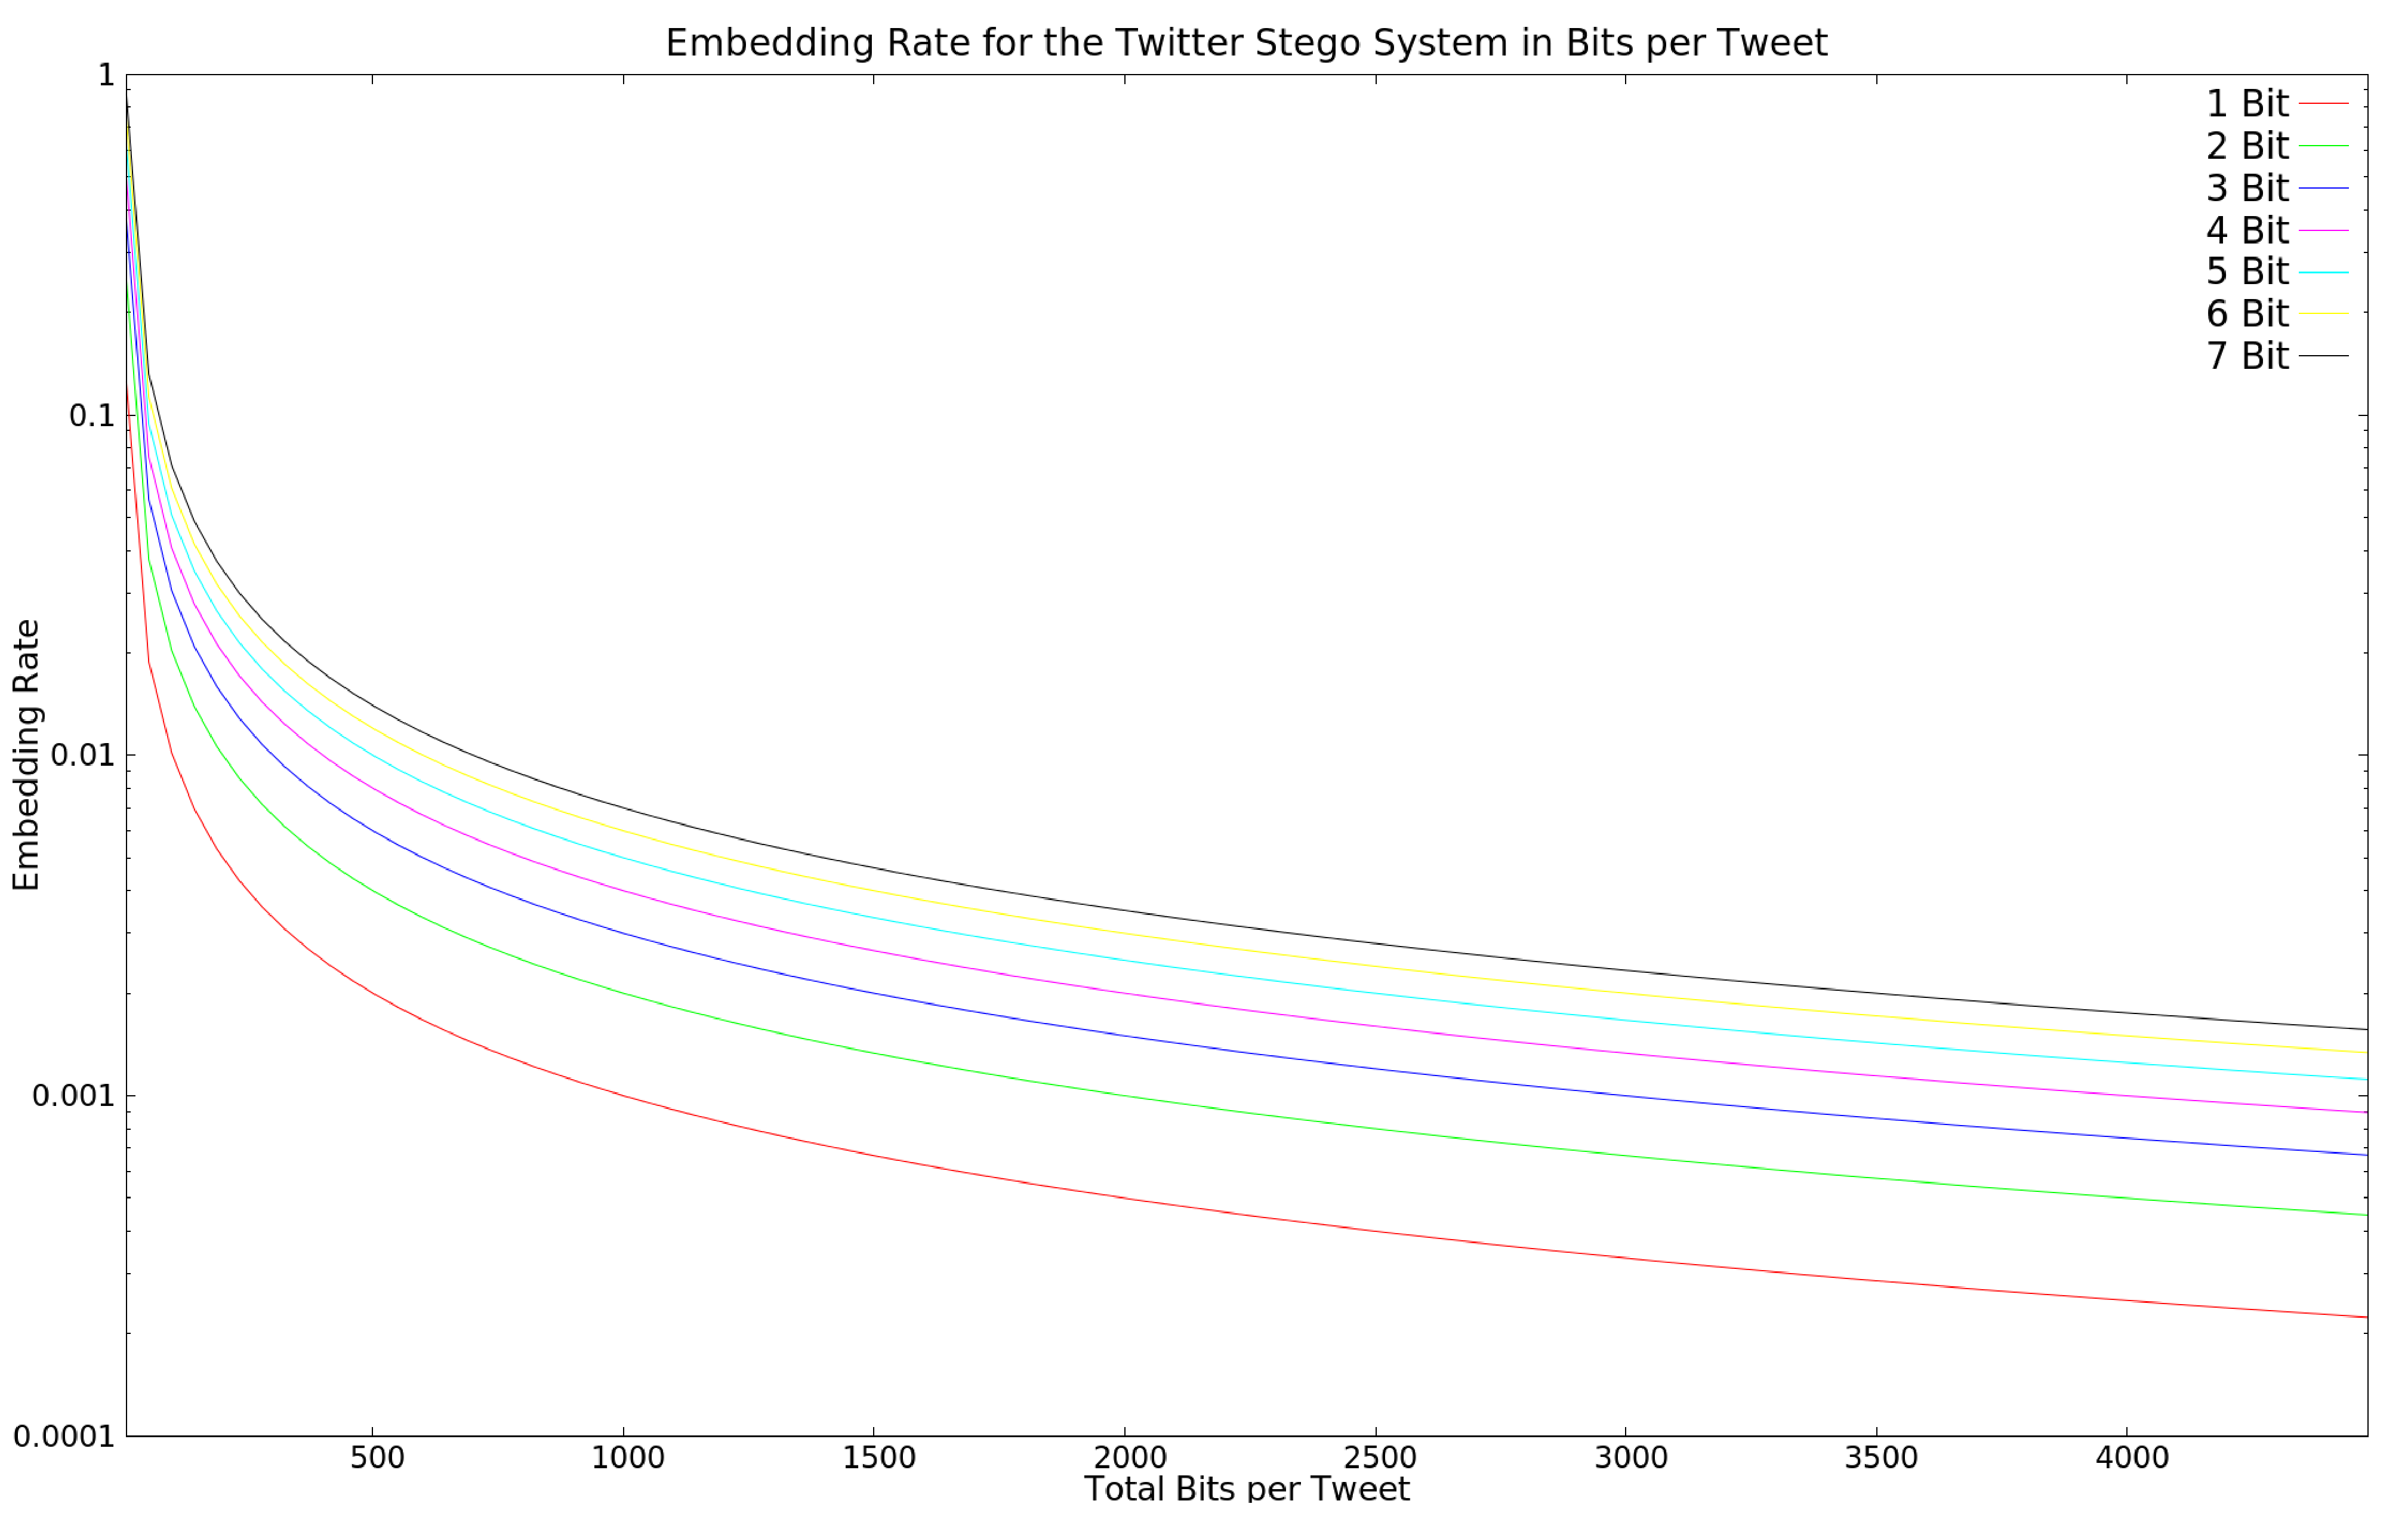
\includegraphics[width=\columnwidth]{embedding-rate.eps}
    \caption{Possible embedding rates for the stego system in bits on a logarithmic scale.}
    \label{fig:evaluation:twittercc:capacity:emebedding-rate}
\end{figure}

Additionally, we must consider how frequently tweets can be posted.  From the
collected Twitter data (see section \ref{sec:methodology:data-collection}),
the time stamp of the tweets was also collected.  For each unique user, the
average number of posts per day was then calculated from this data.  This
data is shown in figure \ref{fig:evaluation:twittercc:capacity:posting-rate}.  In
total, the averege daily posting rate is 8.621 tweets per day.  Therefore, if the
user of the stego system is trying to match real Twitter user posting rates, they
cannot send more than approximately 60 bits of data per day.  If using the system
for botnet command and control, this will allow the botmaster to post a small number
of commands per day.  The botmaster does also have the choice to exceed this
value, but then risks a higher detection rate.  Because the data shows the
average number of tweets posted per day \emph{per account}, that means there
are many accounts that do post more tweets per day.  In this data, there are
several accounts that post on average more than one hundred tweets per day.

\begin{figure}
    \centering
    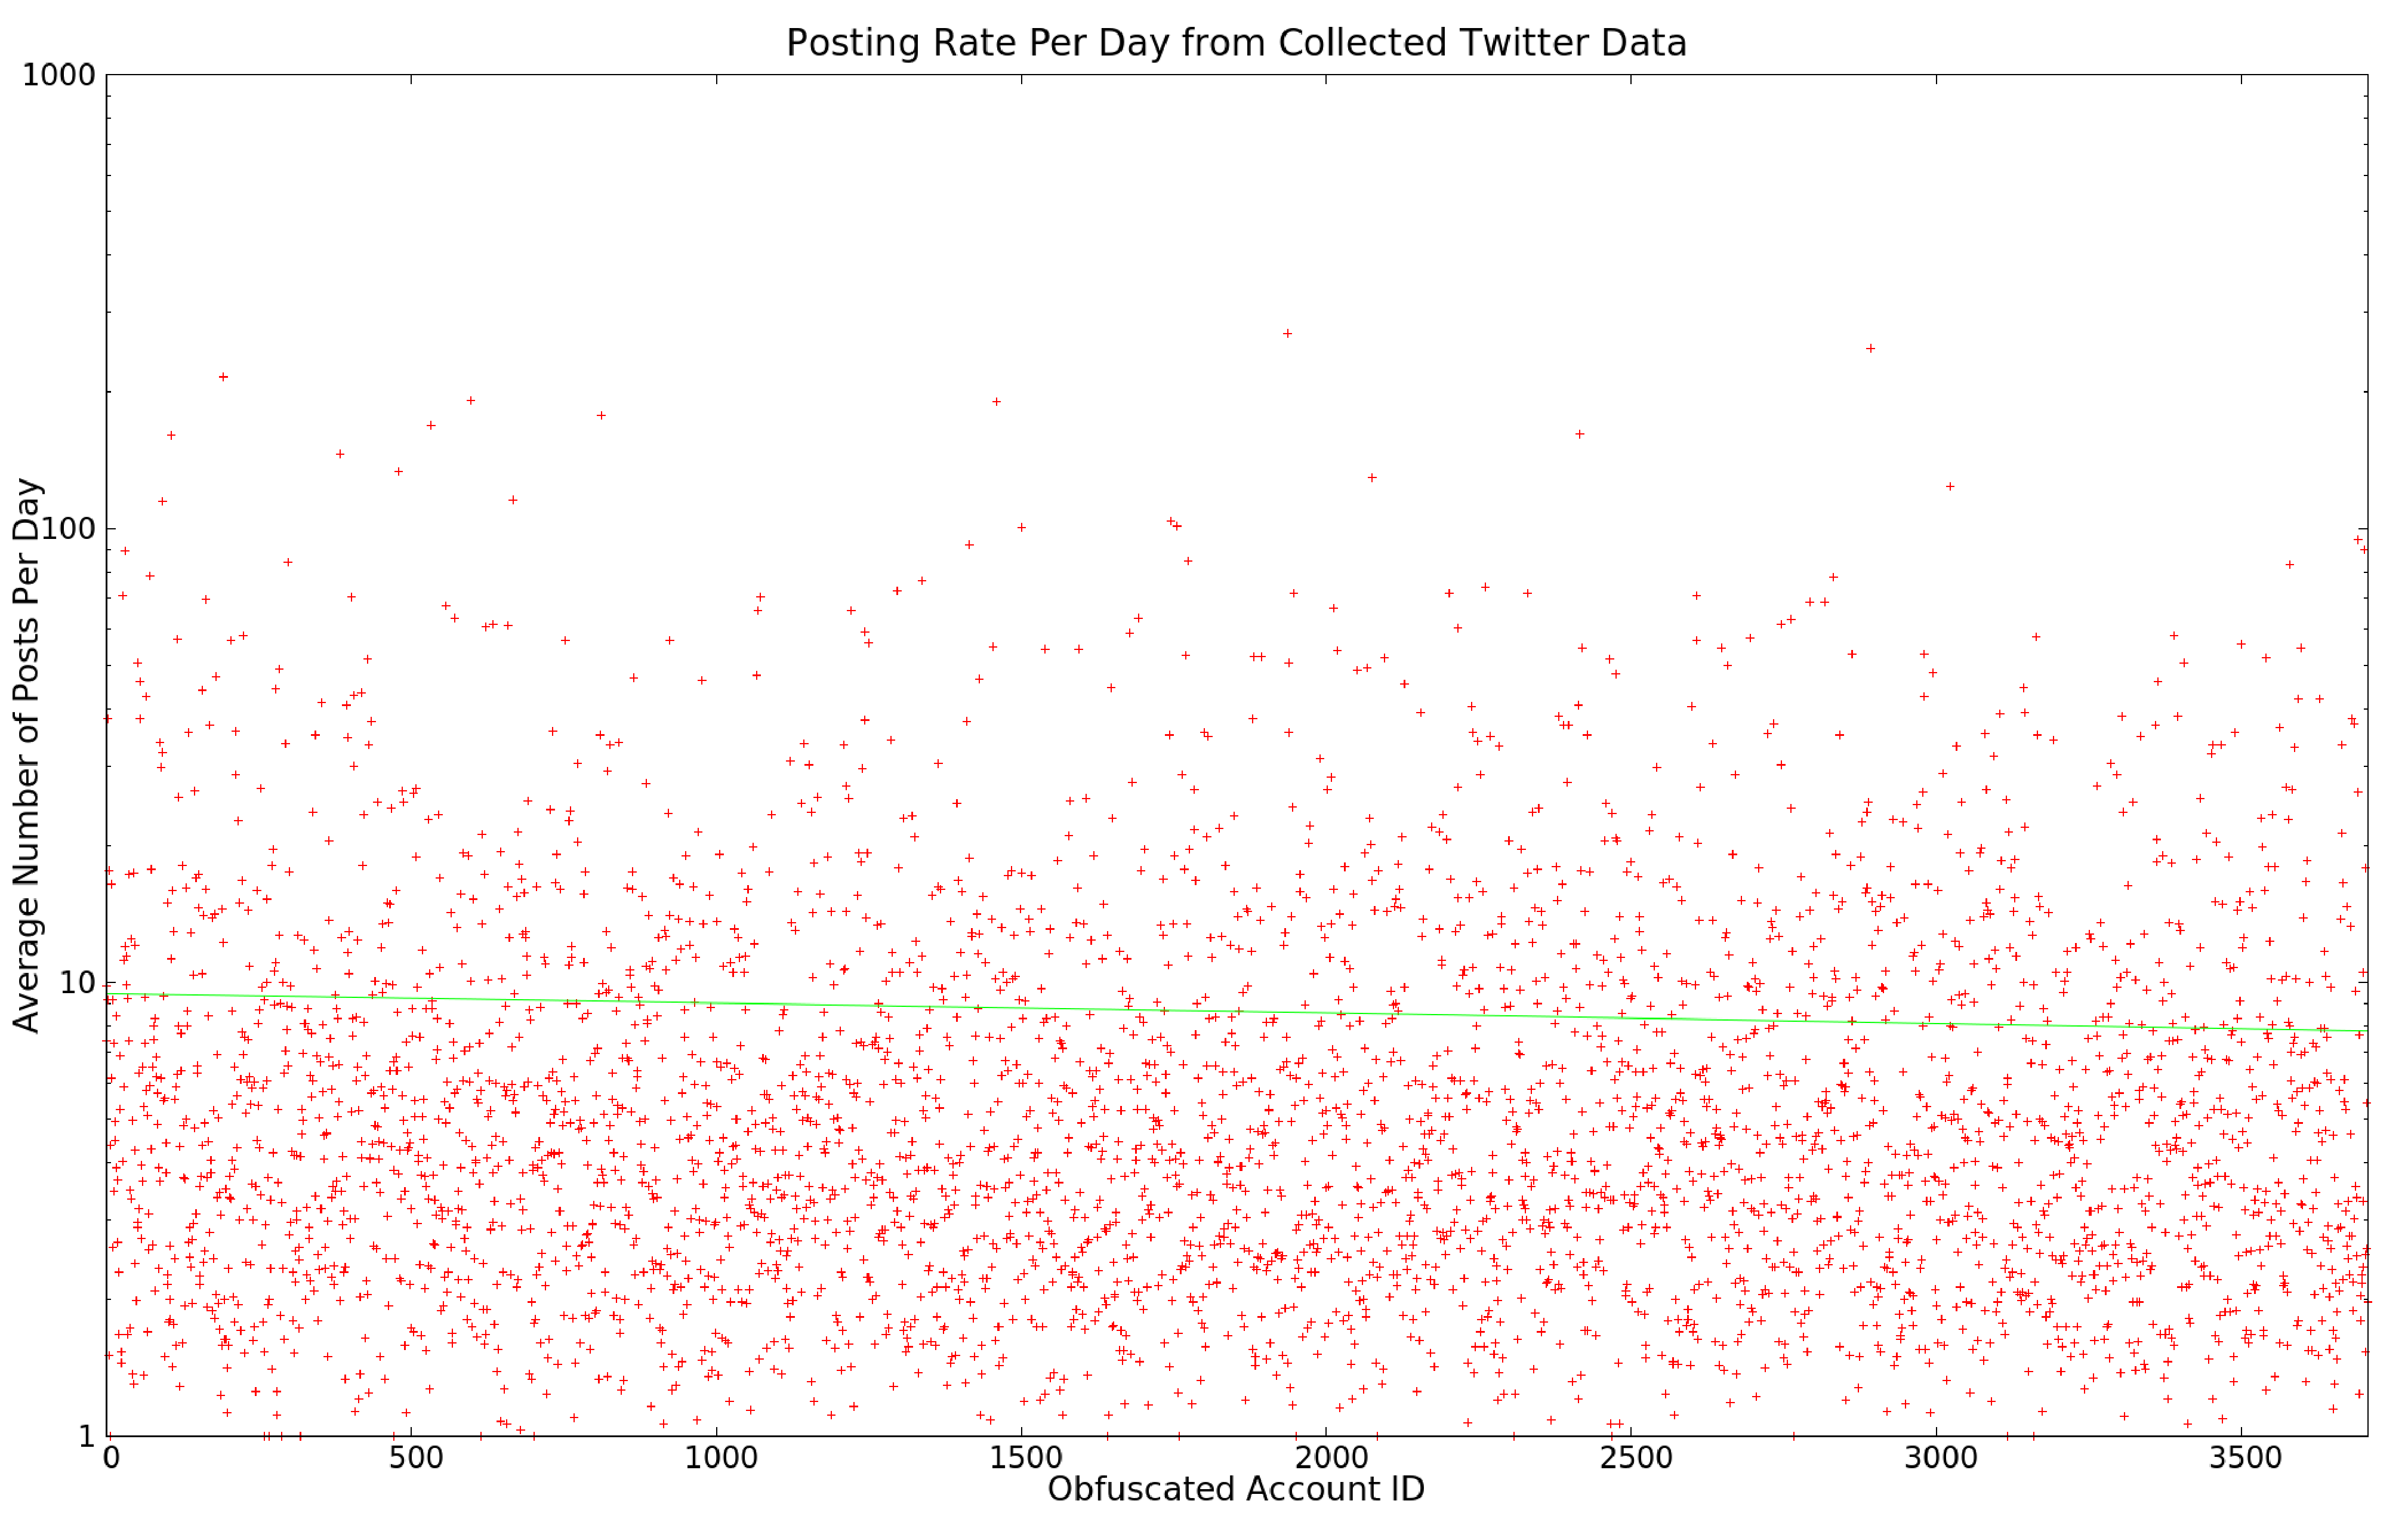
\includegraphics[width=\columnwidth]{posting-rate.eps}
    \caption{Average posting rate in tweets per day on a logarithmic scale.  The green line indicates the mean.}
    \label{fig:evaluation:twittercc:capacity:posting-rate}
\end{figure}

\subsubsection{Steganographic Security}
\label{subsec:evaluation:twittercc:security}

In this stego system we are assuming a \emph{passive warden} model.  In a passive
warden model, an adversary can view each message but cannot modify them.  
The warden must solve the decision problem:
\emph{does this tweet contain a secret message?}  Because our implementation does
not embed any data in to the tweets, most techniques that would be used on a
normal stego system are not sufficient.  The posted tweets appear identical to
any other tweet from a textual perspective.  However, the tweet generation method
is a large determiner of detectability.  It is possible to create the tweets
manually, but if the user wants to send many messages using the stego system
this will be cumbersome.

In order to automate the process, a Twitter bot
program can be used to create the tweets.  An ideal generator would be a
sophisticated Twitter bot that can convince other users that it is human.  This
is similar to passing a Turing test with the Twitter bot.  If an account is
suspected of being a Twitter bot, it does not mean that the communication
has been detected, however it will cause suspicion.  The adversary would have
to recognize that the account is being used to pass secret messages and that
the secret messages are done using the lengths of the tweets.  The adversary
would likely assume that the text somehow contains the secret messages.
If we follow Kerckhoffs' principle \cite{kerckhoffs}, then we must assume the
adversary knows that that the stego system passes messages by tweet lengths.
The two factors that must then be determined are then (i) the account being used for transmission, and (ii) which tweets being posted contain the secret message.


If the adversary has no knowledge of which account is being used, it will
be exceptionally difficult to find.  The Twitter website
states that there are now 271 million active monthly users and over 500 million
daily tweets
posted\footnote{\url{https://about.twitter.com/company}} as of August, 2014.  Because
the tweets have no distinguishing factors in general, an adversary cannot easily
search for the account by tweet content.  If the adversary understands the
tweet generator being used, they may be able to search for the account by the content.
So far, the system has been discussed in a way that implies that all tweets
posted on the account are part of the secret messages, however it is possible
to extend an input alphabet to leave space for ignored tweet lengths.  The Twitter
bot could then post these between tweets that contain actual parts of the
secret messages.

The generator that we used is a database generator, which looks
up tweets of the appropriate length from an existing database.  The database
may be populated by collecting real tweets from other accounts or from collecting
text from other sources.  Two of these database based generators were created.
The first uses a small set of common phrases and for longer tweets some proverbs
were collected from the Internet.
The second uses the Twitter data previous collected (see section
\ref{sec:methodology:data-collection}).  Samples from each of these generators
are shown in table \ref{tab:evaluation:twittercc:security:db-samples}.

\begin{table}
    \centering
    \begin{tabular}{|c|l|l|}
        \hline
        Length & Phrase Generator & Database Generator \\
        \hline
        10 & Lunch time & no ragrets \\
        \hline
        11 & Hello World & I'm so..... \\
        \hline
        12 & Good Morning & @J\_Baxt16 14 \\
        \hline
    \end{tabular}
    \caption{Sample tweets from the database based tweet generators.}
    \label{tab:evaluation:twittercc:security:db-samples}
\end{table}

\subsubsection{Network Packet Analysis}
In addition to analyzing the stego system content on Twitter, a small experiment
was performed using Wireshark\footnote{\url{https://www.wireshark.org/}} to
monitor packet contents while accessing Twitter.  Twitter allows connecting
through HTTPS to access user pages, so when using this system it is best
to always access with HTTPS.  In this experiment, the \ttf{wget} command was
run twice.  First, it was run to access another known Twitter account,
\emph{@BarackObama}.  Then, it was run to access the test account used for
this work, \emph{@alicesend}.  In both cases, the HTML content of the user's
page was downloaded and Wireshark monitored all traffic between the two hosts.
After searching the wireshark packet contents, there is no noticable difference
in the network traffic.  Searches were conducted for identifying strings such
as ``alice'' and ``Obama'' but all application data was encrypted using TLS 1.2
according to Wireshark.  Therefore, this traffic information is insufficient
for determining which accounts are being viewed by the source host.  To a
network observer, it simply appears as regular Twitter traffic, which is
generally common due to Twitter's popularity.

\subsubsection{Robustness}
\label{subsec:evaluation:twittercc:robustness}

Robustness is based on extracting the secret messages from the cover objects
\cite{steganalysis}.  As shown in the Emulab experiment in section
\ref{subsec:evaluation:twittercc:capacity}, aside from some anomalous entries,
every bot decoded the appropriate input symbols perfectly.  This assumes a
passive warden model where no one has tampered with the data in transit.  In an
active warden scenario, there are two possibilities: (i) Twitter is modifying the tweets as they are posted or (ii) an adversary has taken control of the botmaster's Twitter account.

The first scenario is extremely unlikely.  Twitter does perform some modification
as described in section \ref{subsec:evaluation:twittercc:capacity} where trailing
\\whitespace was removed before the tweets were posted.  However, this modification
is well defined and is not intended to modify the contents of the secret or
cover messages.  It can be handled by properly implementing the tweet generator.
The second condition would be devastating for the system.  In most of the paper,
a passive warden model was assumed because it was assumed that the botmaster could
maintain control of their Twitter account.  It is possible that the account is
taken down if Twitter discovers that it is a bot or that some other party obtains
control of the account.  

Aside from the steganographic robustness, the robustness of the system in general
is largely dependent on Twitter's infrastructure,
which is one of the advantages of using such a service as the communication
medium.  In previous years, Twitter has suffered with outages, however it has
recently improved significantly.  Because of Twitter's business model, downtime
is very costly for many corporations, organizations, and individuals that rely
on Twitter for marketing\footnote{\url{http://www.cnet.com/news/the-cost-of-twitter-downtime/}},
giving them great incentive to ensure that service is maintained.

\subsection{Username Generation Analysis}
\label{sec:evaluation:usernames}

\subsubsection{Scoring Names Based on the Generated Markov Chain}
\label{subsec:evaluation:usernames:score-by-Markov}

One of the components in the botnet command and control system is a method
of generating plausible Twitter user names.  As described in section
\ref{sec:methodology:usernames}, Markov chains were used to generate such
user names.  In order to analyze the usernames generated from these Markov
chains, two experiments were performed.  First, a probability measure
was calculated on names based on the Markov chain.  We calculate the probability
that a given string would have been generated by the Markov chain.  Let $N$ be
a name consisting of the sequence of characters $n_1n_2\ldots n_k$.  The
probability, $P(N)$, of choosing $N$ from the Markov chain is then
\begin{equation}
\label{eq:evaluation:usernames:prob}
    P(N) = P(n_1)\times P(n_2 \mid n_1) \times \cdots \times P(n_k \mid n_{k-1})\mbox{.}
\end{equation}
Because Markov chains are ``memoryless'' in that the next state is entirely
dependent on the current state, it is not necessary to factor in previous
choices in the probability calculation.  The result of equation
\ref{eq:evaluation:usernames:prob} becomes small very quickly because of
the number of possibilities, so the answer is stored in log-probability space.
That is, the actual calculation is as follows:
\begin{equation}
    \label{eq:evaluation:usernames:log-prob}
    \log P(N) = \log P(n_1) + \log P(n_2 \mid n_1) + \cdots + \log P(n_k \mid n_{k-1})\mbox{.}
\end{equation}
The score of a name is then calculated as the negative log-probability of the name.
Therefore, a lower score is considered a better name according to the Markov chain.
The Markov chain was constructed based on real name statistics, so if a name
has a higher probability of occurring according to the Markov chain, it should
appear to be a plausible name.

An experiment was run that computed these name scores for all 1.5 million names
collected from Twitter along with the same number of names generated by the
Markov chain, each name having the same length as one of the names from the
original set and also a set of the same number of equally-lengthed random text
names.  The average scores calculated from this experiment are presented in
figure \ref{fig:evaluation:usernames:average}.  Some sample names from each
category are presented in table \ref{tab:evaluation:usernames:samples}.  Keep
in mind that a lower score correlates to a \emph{higher} probability of being
generated by the Markov chain.

\begin{figure}
\centering
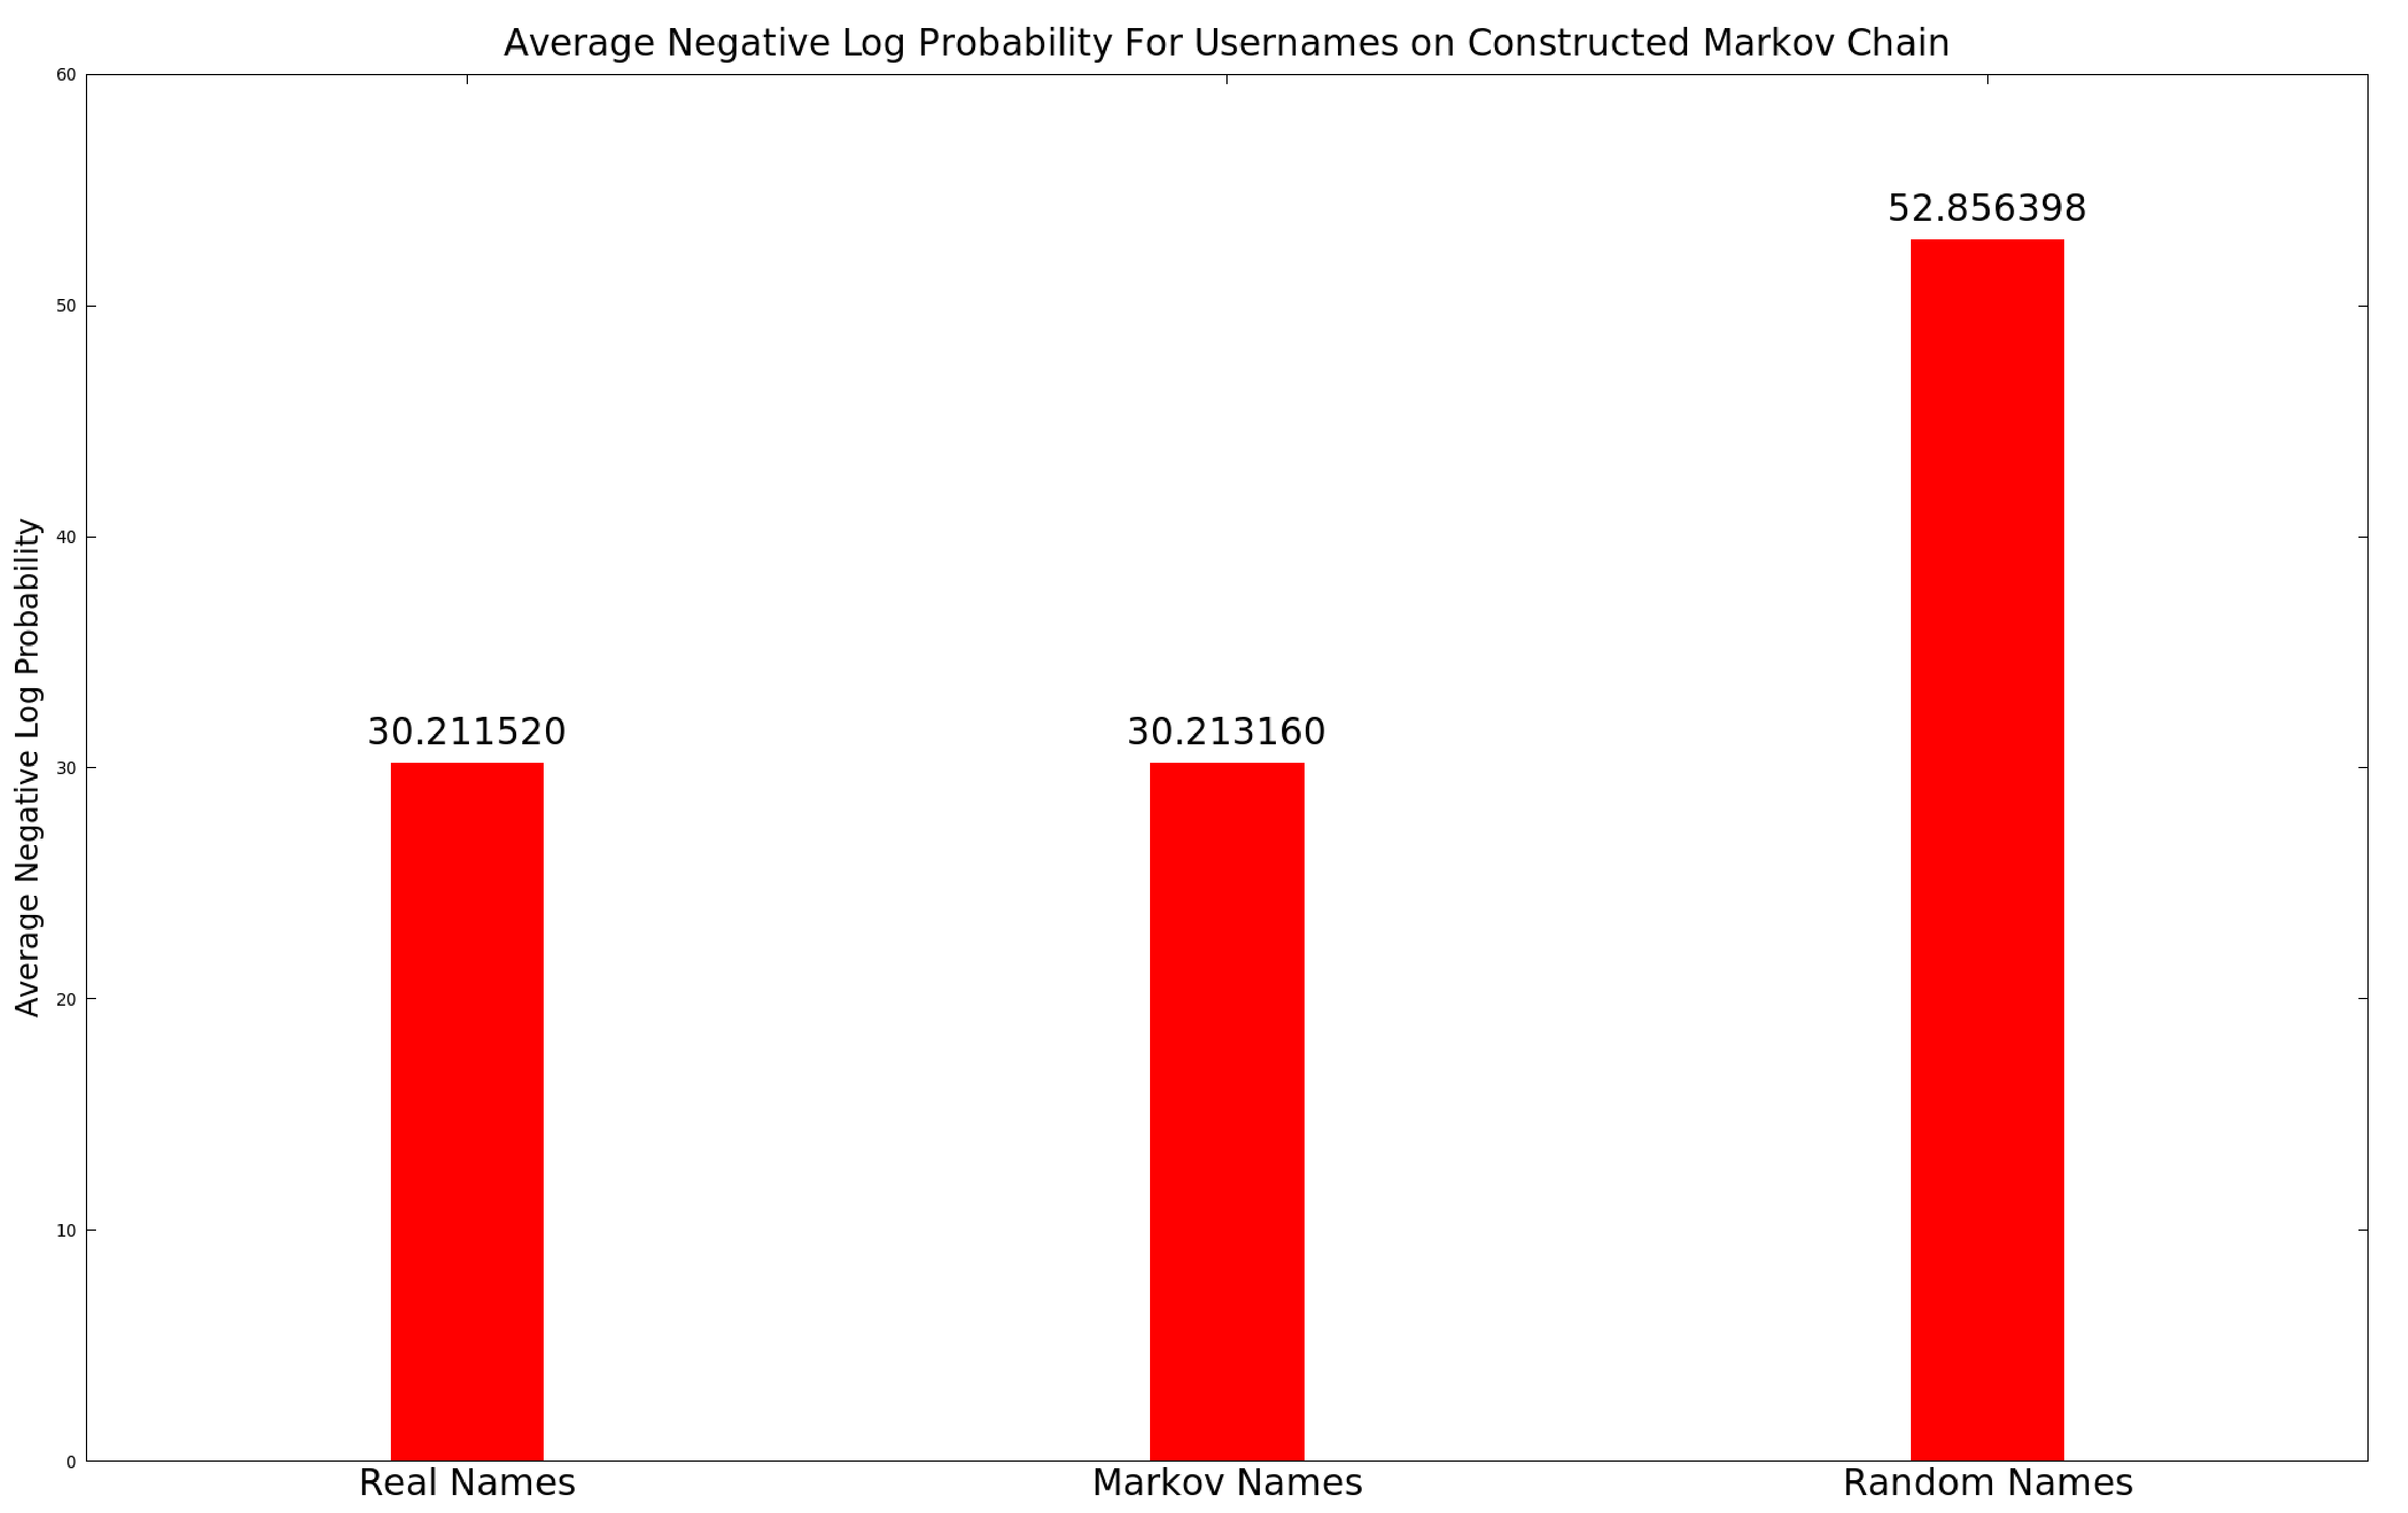
\includegraphics[width=\columnwidth]{usernames-average.eps}
\caption{Average negative log probability score for usernames based on constructed Markov chain.}
\label{fig:evaluation:usernames:average}
\end{figure}

\begin{table}
    \centering
		\resizebox {\columnwidth} {!} {
    \begin{tabular}{|lr|lr|lr|}
    \hline
    \multicolumn{2}{|l|}{Real Usernames} & \multicolumn{2}{l|}{Markov Chain Usernames}
    & \multicolumn{2}{l|}{Random Text Usernames} \\
    \hline
    Name & Score & Name & Score & Name & Score \\
    \hline
    davepeck & 20.189543 & Coccpthe & 24.123132 & wBc3HLqy & 44.472027 \\
    nytimes & 19.178421 & JorayLa & 17.191901 & gzQbhCT & 33.078578 \\
    focuspolitik & 31.618525 & beteckucovao & 30.477696 & KvJhlRwF4G45 & 67.152348 \\
    MarsHill & 20.768233 & Diajan\_m & 20.492829 & PthGonXE & 30.381789 \\
    Scobleizer & 26.922820 & Boumezzost & 25.873167 & vLdHuXVqDO & 56.543208 \\
    warrenellis & 24.335242 & shltirreaha & 30.877799 & 4ok1MwHzWD1 & 60.301202 \\
    redjumpsuit & 32.200608 & SEMarannesi & 25.831416 & QzFS7n4StQt & 58.562229 \\
    joshspear & 23.335631 & McolitePa & 23.613131 & ZhZ1B28vX & 46.774850 \\
    FUELTV & 21.209548 & tudwpi & 20.180779 & hFIn6O & 23.278177 \\
    fredwilson & 27.280397 & MarassttyM & 21.652989 & \_\_hKc4vhHi & 50.487769 \\
    \hline
    \end{tabular}
		}
    \caption{Sample names from each category and their scores.}
    \label{tab:evaluation:usernames:samples}
\end{table}

These results show that names generated by the Markov chain are statistically
identical (within 0.002) to the real usernames used to create the Markov chain.
It is unlikely that an automated system could distinguish between them.  Random
text, however, will not work in this case.  Randomly generated names appear
significantly different than real user names.

\subsubsection{Scoring Names using Human Analysis with Mechanical Turk}
\label{subsec:evaluation:usernames:mturk}

In addition to the statistical analysis, an experiment was performed using Amazon's
Mechanical Turk\footnote{\url{https://www.mturk.com}} system.  The Mechanical Turk
system is a way to connect experimenters that need a human to evaluate something
with willing participants that can perform the evaluation for a small fee per task.

For our experiment, we chose the sentiment analysis template.  This asks users
to choose from one of five choices and provides some more specific instructions
about each choice.  Each worker was shown one user name that is either a real user
name from Twitter, a name generated by our Markov chain, or a name that is just
random text.  The worker did not know from which group the name appeared.  

Essentially, we asked them to
score their confidence in recognizing whether or not the name was real.  If
they were confident that it was fake, they should have answered in the negative.
If they were confident that it was real, they should have answered in the positive.
If they were not sure, they should have answered neutral.  The negative responses
are scored with either -1 or -2 depending on their degree of confidence and the
positive responses are scored with either 1 or 2 depending on their confidence.
A neutral response scores 0.  Each worker was compensated \$0.10 for each name
they scored.  It should be noted that this experiment is exempt from IRB
approval because no identifying information about any participants is collected.
In fact, Mechanical Turk does not provide a way for requesters to identify workers.
Instead, each worker has a pseudonymous user ID number.  Participants were only
asked to respond to a survey of their opinions about the validity of the user names,
not even the user ID was collected after the experiment was performed.

In total, 50 names were chosen from each category and each name
was shown to five different workers.  The aggregated results are shown in figures
\ref{fig:evaluation:usernames:real-mturk-agg}, \ref{fig:evaluation:usernames:Markov-mturk-agg},
and \ref{fig:evaluation:usernames:random-mturk-agg}.  

\begin{figure*}
\begin{minipage}{0.3\textwidth}
        \centering
    \centering
    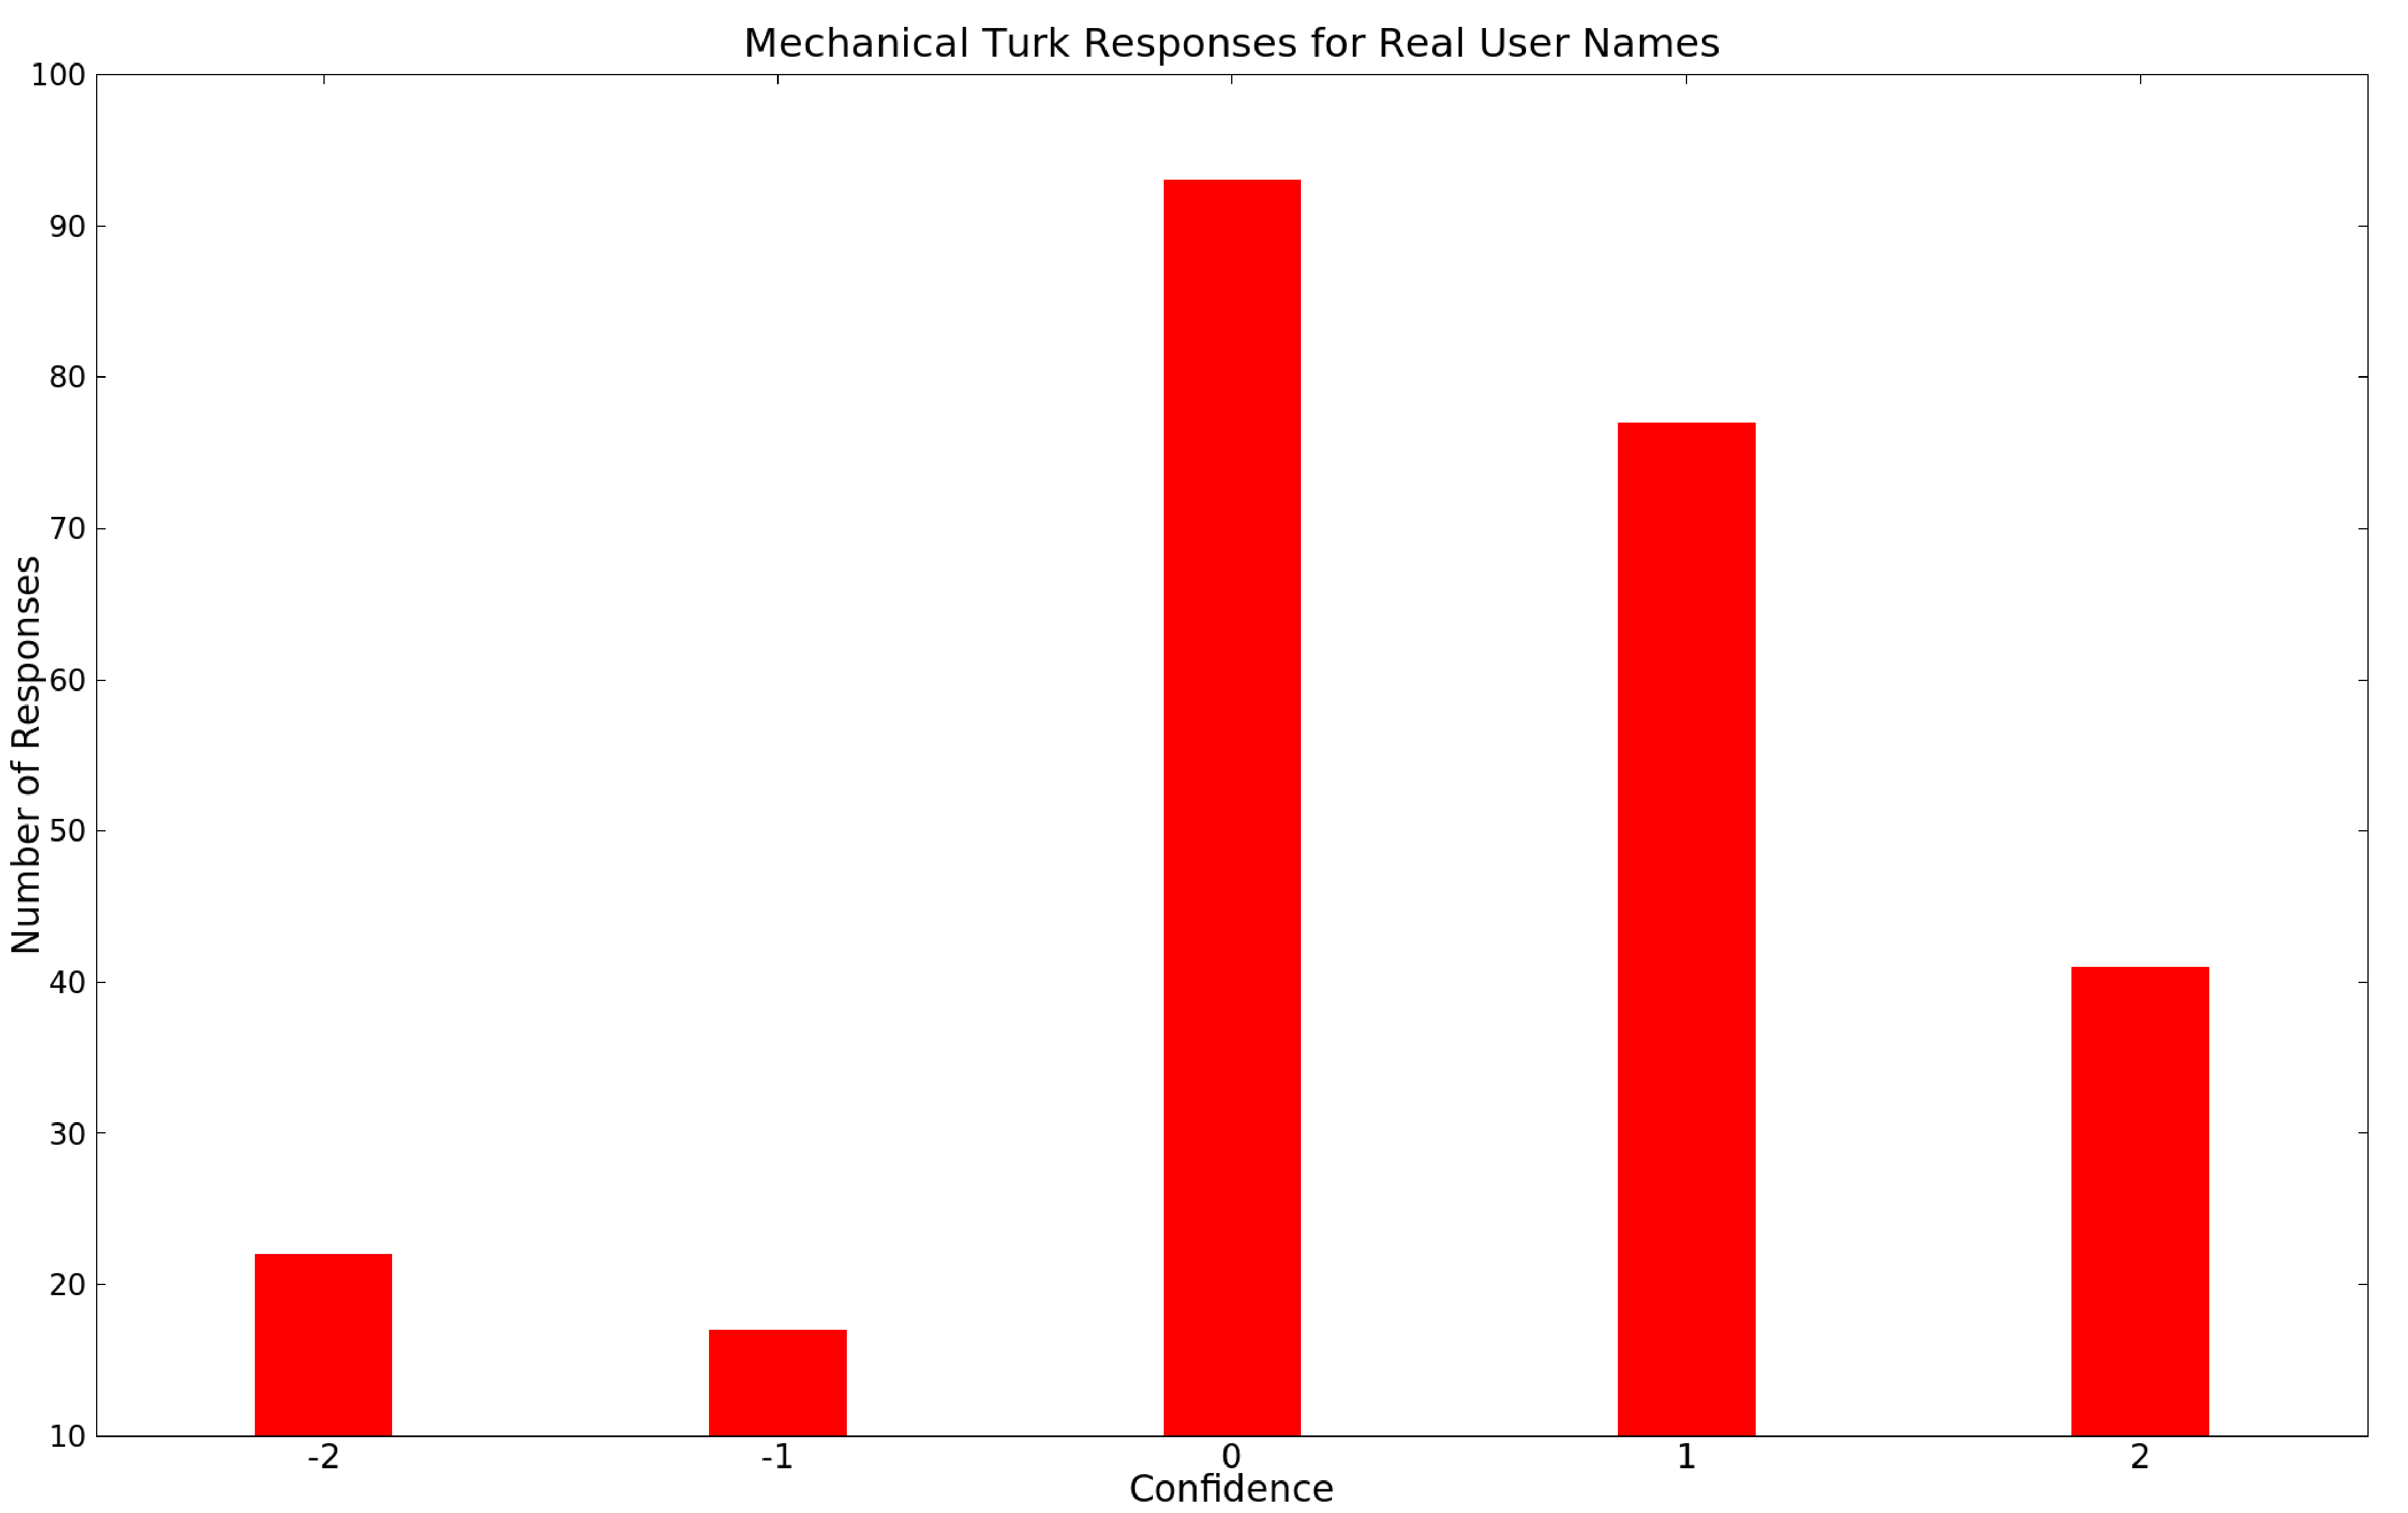
\includegraphics[width=\columnwidth]{real-mturk-agg.eps}
    \caption{Aggregate scores for real usernames from the Mechanical Turk experiment.}
    \label{fig:evaluation:usernames:real-mturk-agg}
\end{minipage}%
\hspace{5mm}
\begin{minipage}{0.3\textwidth}
        \centering
					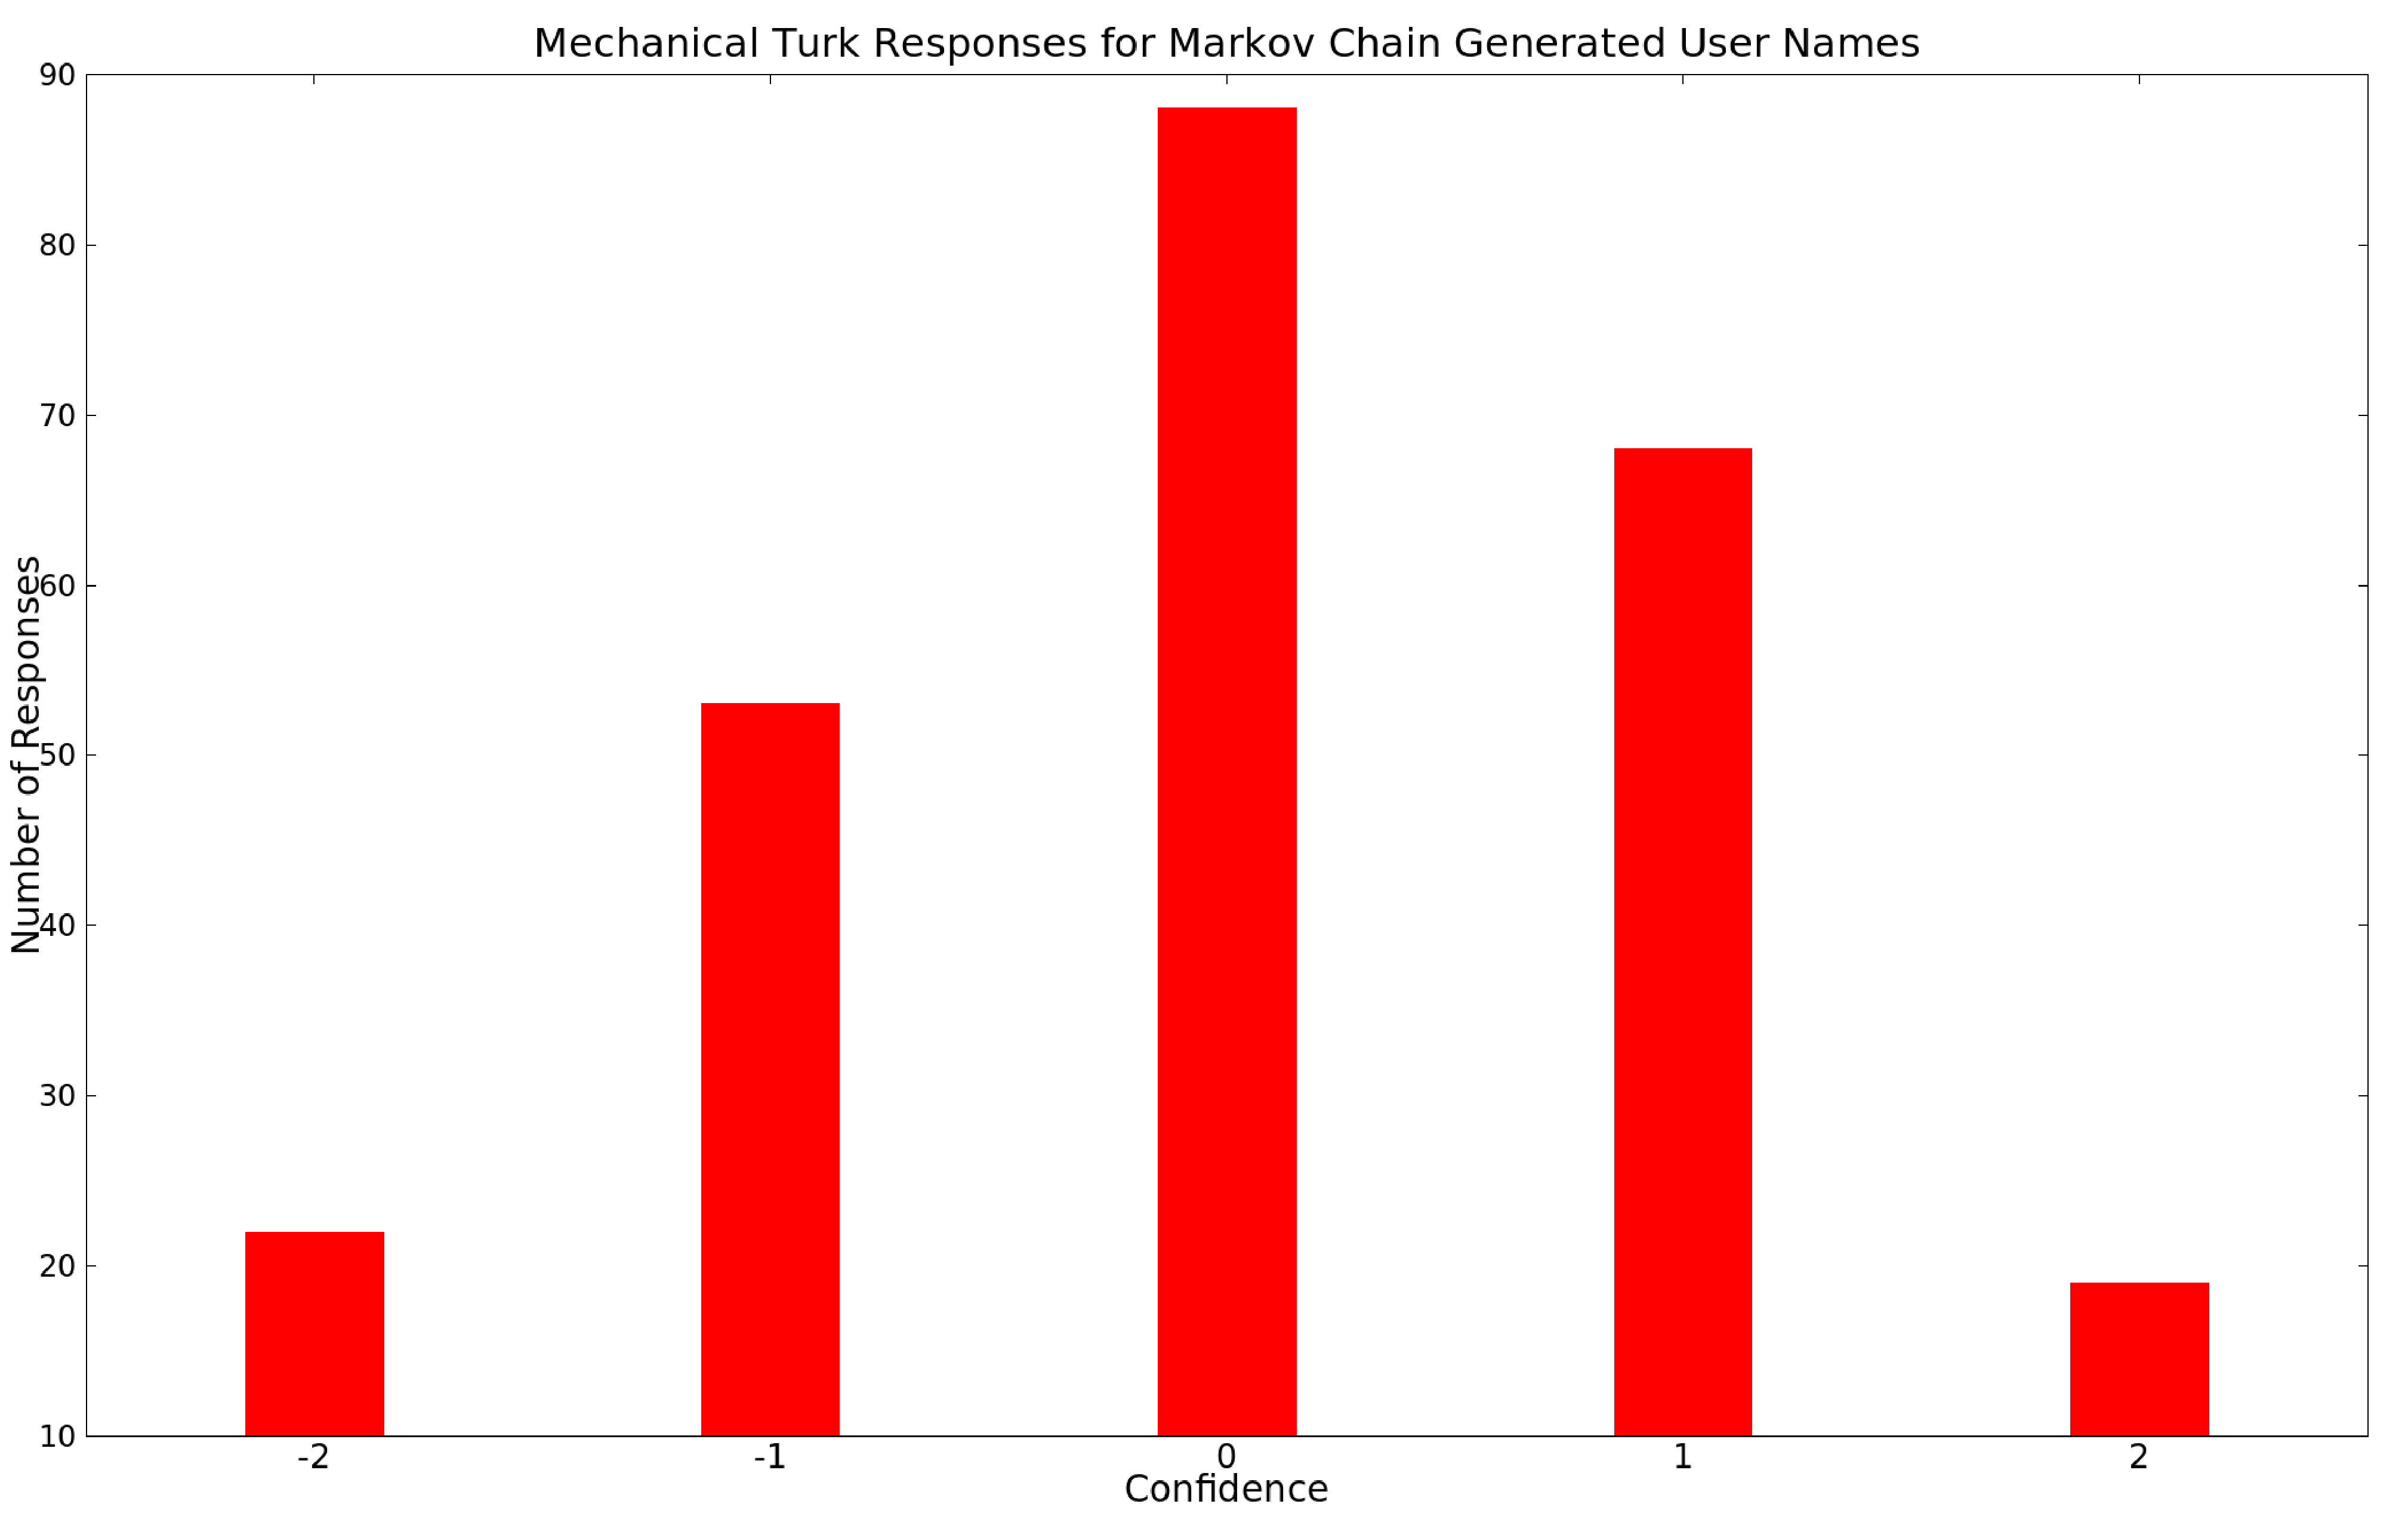
\includegraphics[width=\columnwidth]{Markov-mturk-agg.eps}
    \caption{Aggregate scores for Markov chain generated usernames from the Mechanical Turk experiment.}
    \label{fig:evaluation:usernames:Markov-mturk-agg}
\end{minipage}%
\hspace{5mm}
\begin{minipage}{0.3\textwidth}
        \centering
    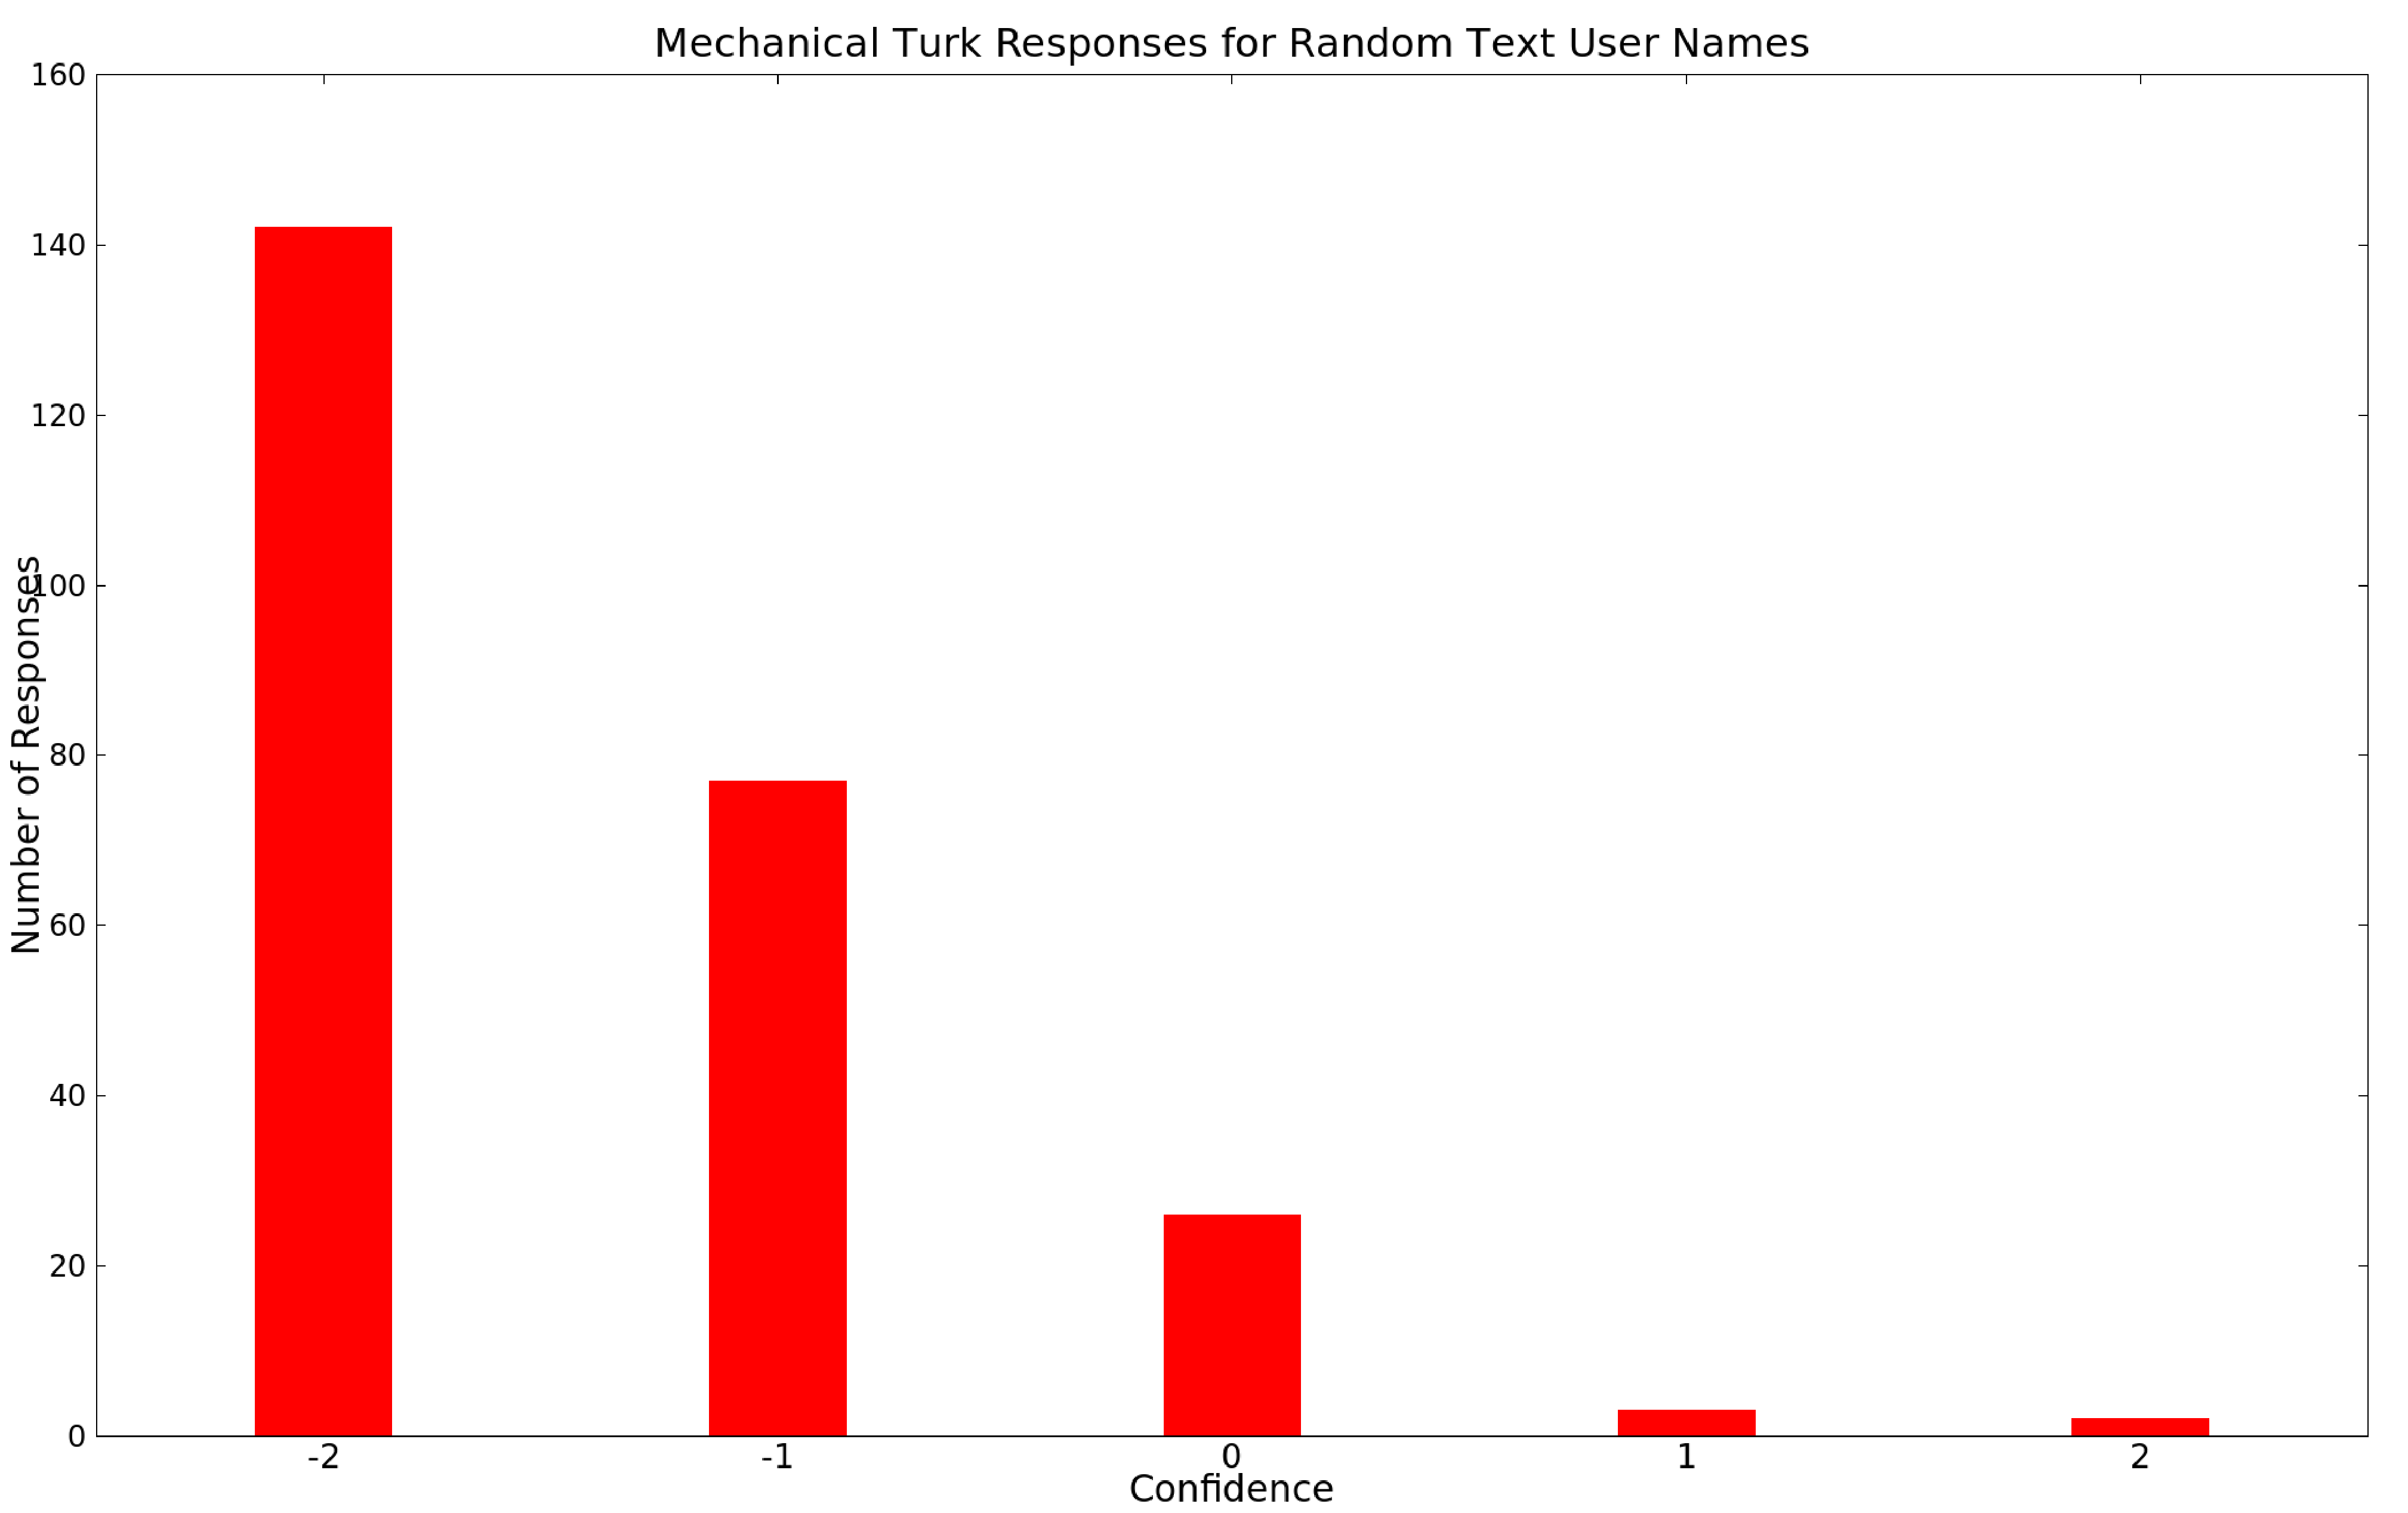
\includegraphics[width=\columnwidth]{random-mturk-agg.eps}
    \caption{Aggregate scores for random text usernames from the Mechanical Turk experiment.}
    \label{fig:evaluation:usernames:random-mturk-agg}
\end{minipage}
\end{figure*}

These results show some differences compared with the automated statistical
analysis above.  Random names, however, appear obviously fake to human examiners.
Almost all responses for the random names were negative.  It does appear, though,
that humans are not confident in recognizing real names either, with a plurality
of results being zero and some negative.  They seem to have some inclination toward
recognizing fake names generated by the Markov chain, with more negative answers
than the real user names, but very few considered themselves very confident (a score of -2).

The results from both the statistical analysis and the Mechanical Turk survey
indicate that the method being used for username generation is sufficient to
create usernames that would not appear abnormal to either an automated name
analysis tool or to human users viewing the page on Twitter.  Therefore, this
method can be used as the username generation method for a botnet that must
create a new account and switch communications to it for some reason, e.g.\ if
Twitter blocks the previous account.  By starting with a common seed, each bot
can generate the appropriate new name and connect to the new account.
